\chapter{插图}\label{sec:graphics}

\begin{quotation}
A picture says more than a thousand words.
\begin{flushright}
--- Shakespeare
\end{flushright}
\end{quotation}

当年Knuth开发 \TeX 时,GIF, JPEG, PNG, EPS 等图形格式还没有问世,所以 DVI 不能直接支持这些格式。但是高手就是高手,Knuth 在 \TeX 里留了一个后门:\verb|\special| 命令,让后面的驱动自行决定怎样处理图形。

这和当年老毛把港澳台,老邓把钓鱼岛都“留给后人解决”有异曲同工之妙。曾经有位出版社的编辑看上了包老师写的一个程序,要我改改当作教学辅助软件出版,但是当时手头没有DOS中断的资料没办法加鼠标操作。该编辑说:你把鼠标驱动打包在软件里,让用户自己琢磨是怎么回事。

下面我们会在 \ref{sec:graphics_format} 节讨论 \LaTeX 所用图形格式以及图形的优化、转换和处理,\ref{sec:includegraphics} 节介绍怎样插入图形,\ref{sec:draft} 节简介矢量绘图。接下来的六至八章会分别讨论怎样使用 \MP, PSTricks 和 PGF。

\section{图形概览}
\label{sec:graphics_format}

\subsection{图形格式}

\LaTeX 支持点阵图形格式 JPEG 和 PNG,也支持矢量格式 EPS 和 PDF \footnote{EPS 和 PDF 中也可以嵌入点阵图形,但是它们本身还是矢量格式。}。对于示意图,我们应该首选矢量格式;包含大量自然色彩的图像 (比如照片) 应该选 JPEG;人工点阵图像应该选 PNG。

1980年代中后期,PostScript 风头之劲一时无两,人们自然会考虑把它作为文档中嵌入图形的标准格式。然而它实在太强大,人们担心嵌入文档的 PostScript 会搞破坏,于是就产生了戴着手铐的 Encapsulated PostScript (EPS) 。出于同样的原因,人们也担心嵌入 HTML 的 ActiveX, Java Applet, JavaScript 中混入恶意代码,所以才会对它们也有所限制。早年间人们得到 DVI 后通常会把它转换为 PostScript,所以 EPS 就成了 \LaTeX 的标准图形格式。
 
\subsection{Driver的口味}

\subsubsection{dvips}

\texttt{dvips} 喜欢 PostScript,所以就爱屋及乌只支持嵌入 EPS。MiKTeX 看不惯这种垄断行为,就把 \texttt{dvips} 破解,添加了对 JPEG 和 PNG 的支持。但是它很固执,坚持按缺省分辨率72 PPI计算图形尺寸,并认为所有图形都是灰度图。为了避免麻烦,包老师还是劝你把这些图形格式转换为 EPS。

\subsubsection{pdflatex}
\texttt{pdflatex} \footnote{\texttt{pdflatex} 包含编译和驱动两种功能,所以这里也就把它划到驱动一边。} 支持 JPEG, PNG 和 PDF,不支持 EPS。传说它不支持 EPS 的原因是 PostScript 解释器的版权问题。包老师认为这种说法不可信,因为1997年 pdfTeX 面世时 PostScript 已经被 PDF 赶超,Adobe 与其保护 PostScript 还不如保护 PDF。

\LaTeX 有两个宏包 \texttt{epstopdf} 和 \texttt{pst-pdf} 可以实时地 (on the fly) 把 EPS 转换为 PDF \footnote{在这里 on the fly 是指在后台处理,用户不用操心。包老师不确定把它翻译为“实时”是否合适,因为 real time 通常被翻译为实时。对于用户无须干涉、知情的情况,有人说 user transparent,也有人说 black box,语言还真奇妙。}。然而前者有安全漏洞,后者用法繁琐,用户最好还是用其他软件事先把 EPS 转为 PDF。

\subsubsection{dvipdfm(x)}

\texttt{dvipdfm} 支持 JPEG, PNG 和 PDF,不支持 EPS,但是它可以实时地调用 Ghostscript 把 EPS 转为 PDF。\texttt{dvipdfmx} 对上述图形格式的支持有所增强,还增加了对 BMP 的支持。

\subsubsection{xdvipdfmx}

\XeLaTeX 的缺省驱动 \texttt{xdvipdfmx} 直接支持 BMP, JPEG, PNG, EPS 和 PDF。所以从图形格式支持的角度来讲,\texttt{xdvipdfmx} 比 \texttt{dvips, pdflatex} 和 \texttt{dvipdfmx} 都好。传说 \texttt{xdv2pdf} 驱动还支持 GIF, PICT, PSD, SGA, TGA, TIFF 等格式,可惜只能在 Mac OS X 上用。

\subsection{图形优化}

矢量图形的一个优点是可以无限缩放,而输出质量不变。图形尺寸对矢量图形而言意义不大。描述矢量图形所需数据较少,所以其文件体积一般也较小。

而点阵图形是以像素 (pixel) 为单位描述、存储的,图形尺寸越大,文件体积就越大。当然影响文件体积的还有色彩深度、压缩算法等因素。

人们一般希望用较小的文件体积获取较好的输出效果,这样就需要优化图形尺寸和色彩。

\subsubsection{图形尺寸}

点阵图形的像素是一种相对尺寸,其实际尺寸等于像素除以分辨率 (resolution) ,最常用的分辨率单位是像素/英寸 (pixels per inch,PPI) 。在古时候PPI也常和点/英寸 (dots per inch, DPI) 混用;现在人们倾向于认为 PPI 是图形的分辨率单位,而 DPI 是硬件设备 (比如显示器或打印机) 输出的分辨率单位。通常横向和纵向分辨率相同,可以写成一个数字。

比如有一幅100 × 150像素的点阵图形 (\autoref{fig:default_size}) ,其分辨率为100 PPI。在输出时,它的缺省尺寸就是 1in × 1.5in。如果我们将它强制输出为 2in × 3in (\autoref{fig:force_size}) ,那么其实际分辨率就降为 50 PPI。

\begin{figure}[htbp]
\centering
\begin{minipage}[b]{1.4in}
\centering
\includegraphics{anna.jpg}
\caption{缺省输出尺寸}
\label{fig:default_size}
\end{minipage}
\hspace{10pt}
\begin{minipage}[b]{2in}
\centering
\includegraphics[width=2in]{anna.jpg}
\caption{强制放大输出尺寸}
\label{fig:force_size}
\end{minipage}
\end{figure}

假设输出分辨率是 100 DPI,像素和输出点就一一对应;如果输出分辨率是 300 DPI,每个像素实际输出为3 × 3个点;如果输出分辨率是 50 DPI,每2 × 2个像素才享受到一个输出点的待遇。

当图形分辨率和输出分辨率不一致时,就会有一个重新采样 (resampling) 的过程;从高分辨率到低分辨率叫下采样 (downsampling) ,反之叫上采样 (upsampling) 。重新采样的插值 (interpolation) 算法有很多,其中常用的有最近像素 (nearest neighbor) 、双线性 (bilinear) 、双三次 (bicubic) 、兰索斯 (Lanczos) 等。前两种速度快,但是效果差;后两种效果好,但是速度慢。追求完美的雷人自然要选择 Lanczos。

一般而言,高分辨率图形配合高分辨率输出设备会产生高质量效果,低分辨率图形配合低分辨率设备会产生低质量效果;高分辨率图形遇到低分辨率设备会形成浪费;低分辨率图形遇到高分辨率设备呢,得看插值效果,但是最好嫑高估机器的智能。雷人追求的是高质量文档,所以输出设备的分辨率大家暂时就甭操心了。

当输出尺寸一定时,图形分辨率越高需要的像素就越多,图形文件体积就越大。那么点阵图形的分辨率多少比较合适呢?一般认为在屏幕上阅读需要 72 PPI,考虑到放大 150 PPI 应该够了,而高质量打印需要 300 PPI。

假设我们要在 \LaTeX 文档中嵌入一幅图形,如果是通栏,宽度就是4.8--5.4in (文档缺省宽度取决于字体大小) 。那么如果仅用于屏幕阅读,原始图形的宽度 400px 足够了;如要放大阅读或输出打印则分别需要 800px 和 1600px。

点阵图形尺寸相关的基本编辑操作有以下几种:裁剪 (crop) 、改尺寸 (resize) 、改分辨率。

\begin{enumerate}
\item 裁剪时像素自然会变少,分辨率不变,缺省输出尺寸也就变小。\autoref{fig:default_size} 其实就是从一幅 2048 × 1536 像素的大图裁剪、缩小而来,因为原图太大,\autoref{fig:original} 把它强制输出为 4in × 3in。

\item 改尺寸时像素改变,分辨率不变,缺省输出尺寸相应改变,这个过程需要重新采样。比如把 \autoref{fig:default_size} resize 到 200 × 300 像素,分辨率还是 100 PPI,那么缺省输出尺寸就变成 2in × 3in (\autoref{fig:resize}) 。

\item 单纯更改图形文件分辨率时,像素不变,缺省输出尺寸相应改变。把 \autoref{fig:default_size} 分辨率设为 200 PPI,像素还是 100 × 150,那么缺省输出尺寸就变成 0.5in × 0.75in (\autoref{fig:density}) 。

\item 改尺寸和改分辨率可以结合使用。把 \autoref{fig:default_size} 的尺寸改为 200 × 300 像素,分辨率改为 200 PPI,缺省输出尺寸就还是 1in × 1.5in (\autoref{fig:resample}) 。
\end{enumerate}

\begin{figure}[htbp]
\centering
\includegraphics[width=4in]{dscf6030.jpg}
\caption{原始图形}
\label{fig:original}
\end{figure}

综上所述,点阵图形的信息量取决于像素。图形文件的分辨率只是“建议”缺省输出尺寸,并不影响图形质量。上述操作中裁剪和改尺寸比较实用,改分辨率没有实质意义。改尺寸一般也只能从大改小。如果从小改大的话,插补出来的像素比起原装的还是要差一些。

\begin{figure}[htbp]
\centering
\begin{minipage}[b]{2in}
\centering
\includegraphics{anna_resize.jpg}
\caption{改尺寸}
\label{fig:resize}
\end{minipage}
%\hspace{5pt}
\begin{minipage}[b]{1.1in}
\centering
\includegraphics{anna_density.jpg}
\caption{改分辨率}
\label{fig:density}
\end{minipage}
%\hspace{5pt}
\begin{minipage}[b]{1.6in}
\centering
\includegraphics{anna_resample.jpg}
\caption{改尺寸和分辨率}
\label{fig:resample}
\end{minipage}
\end{figure}

需要指出的是上述操作在不同的软件里名称不同,比如改尺寸,相当于 ImageMagick 中的 resize 和Adobe PhotoShop 中的 resample;改分辨率,相当于 ImageMagick 中的 density 和 PhotoShop 中的 resize;上面第四种混合操作,在 ImageMagick 叫resample。包子曰:道可道,非常道。名可名,非常名。

\subsubsection{色彩深度}

色彩深度 (color depth) 是每一个像素所用颜色的位数。比如一位可以表示两种颜色,通常是黑白;两位可以表示四色,最早用于 CGA 显卡;四位16色,用于 EGA 显卡;八位256色,用于 VGA 显卡;16位65,536色,又称高彩;24位16,777,216色,又称真彩;30--48位称为深彩。

色深位数越高越逼真,文件体积也就越大。一般照片可以用24位,人工图像用八位足矣,图标之类的小图形可以考虑更少位数。从 \autoref{fig:depth} 我们可以看到各种色深的效果和文件体积,它们都是 PNG 格式。

\begin{figure}[htbp]
\centering
\begin{tabular}{ccc}
  \includegraphics{anna.png} & \includegraphics{anna8.png} & \includegraphics{anna8g.png} \\
  24位真彩 34 KB & 8位256色 23.4 KB & 8位灰度 18.7 KB \\
  \includegraphics{anna4.png} & \includegraphics{anna2.png} & \includegraphics{anna1.png} \rule{0pt}{111pt} \\
  4位16色 15.6 KB & 2位4色 13.5 KB & 1位黑白 12 KB
\end{tabular}
\caption{色彩深度}
\label{fig:depth}
\end{figure}

我们一般也只能把图形的色深从高改低,从而减小图形文件和最终文档的体积。反过来把低色深从低改高,属于逆势而为,或遭天谴。

\subsection{图形转换和处理}

按说有了 \XeLaTeX 之后雷人已经基本上不再需要转换图形格式,只是有时出版社会指定使用某几种图形格式;另外我们常常需要优化图形,否则直接嵌入文档有点浪费。这时图形处理软件就派上了用场。

注意把点阵图形转换为矢量图形并不能提高图形本身的质量,正所谓“garbage in, garbage out”。

第一章简介中提到的 Ghostscript 不仅包含 RIP,还提供 PostScript, EPS 和 PDF 等文件格式的转换功能。通常人们会通过 Ghostscript 的一个图形前端来调用它的功能,它最常用的前端是 GSview。

通用图像处理软件种类繁多。如果你喜欢命令行界面包老师推荐 ImageMagick,喜欢图形界面的可以试试 Paint.NET,喜欢凌乱的界面而且内存多得用不完的可以试试 GIMP。其他收费软件有悖于自由软件的精神,这里不提也罢。

\subsubsection{ImageMagick}

ImageMagick 包含多个命令行程序,其中最常用的是 \texttt{convert}。下面的命令把 BMP 转换为 PNG,据说 ImageMagick 可以识别100多种格式。

\begin{Code}[]
convert fig.bmp fig.png 
\end{Code}

Windows 有个用来转换分区格式的同名程序。所以我们在 Windows 下使用 ImageMagick 时,需要写全路径,或者在 \texttt{PATH} 环境变量里把 ImageMagick 的路径放到 \texttt{system32} 前面。

图形尺寸相关操作命令如 \autoref{exa:im_size} 所示。第1行命令裁剪并且转换格式,截取从 (10,10) 开始 300 × 200 像素的图像,原点在左上;第2行裁剪并缩放;第3行缩放到 300 × 200 像素范围内,保持长宽比;第4行强制缩放到给定尺寸,不考虑长宽比;第5行把分辨率改为 300 PPI;第6行把分辨率改为 300 PPI,像素增加,缺省输出尺寸维持不变。

\begin{example}[h]
\begin{Code}[numbers=left]
convert fig.bmp -crop 300x200+10+10 fig.jpg
convert fig.jpg -crop 300x200+10+10 -resize 30x20 fig1.jpg
convert fig.jpg -resize 300x200 fig1.jpg
convert fig.jpg -resize !300x200 fig1.jpg
convert fig.jpg -density 300 fig1.jpg
convert fig.jpg -resample 300 fig1.jpg
\end{Code}
\caption{ImageMagick尺寸操作}
\label{exa:im_size}
\end{example}

图形色深相关命令如 \autoref{exa:im_depth} 所示。第1行命令把图形转为8位256色,第2行转为8位灰度,第3行转为4位16色,第4行转为2位4色,第5行转为1位黑白。

\begin{example}[h]
\begin{Code}[numbers=left]
convert fig.jpg -colors 256 png8:fig8.png
convert fig.jpg -colorspace gray png8:fig8g.png
convert fig.jpg -colors 16 png8:fig4.png
convert fig.jpg -colors 4 png8:fig2.png
convert fig.jpg -monochrome fig1.png
\end{Code}
\caption{ImageMagick色深操作}
\label{exa:im_depth}
\end{example}

ImageMagick 功能强大,参数选项很多,这里只能蜻蜓点水。它有一个缺点,缩小图像做缩略图时不是很清晰;也许可以调整参数改善清晰度。我用过的软件中 ACDSee 做的缩略图最清晰,但它是收费软件。

\subsubsection{其他格式转为EPS}

有很多软件都可以把点阵图像转换为 EPS,比如 ImageMagick 和 GIMP,以及 \href{https://texfaq.org/FAQ-dvipsgraphics}{a2ping/sam2p, bmeps, jpeg2ps, sam2p} 等。

PostScript 从 Level 2 开始才支持点阵图像压缩,所以在把其他格式转为 EPS 时应尽量使用 Level 2 或 3,否则输出的 EPS 会很大。

ImageMagick 转换 EPS 的方法如下。如果是 BMP 文件,最好先压缩成 JPEG 或 PNG,再转为 EPS,这样生成的 EPS 会比较小。我猜 EPS 的缺省压缩算法可能不如 JPEG 和 PNG。

\begin{Code}
convert fig.png eps3:fig.eps
\end{Code}

另一种方法是用虚拟打印机生成EPS,它的优点是可以把几乎所有文件“打印”成 EPS。包老师推荐 Bullzip PDF Printer,它可以把各种文件打印成 PS, EPS, PDF, BMP, JPEG, PCX, PNG, TIFF 等格式。

用合适的软件打开原始文件,打印到 Bullzip PDF Printer。在 General 标签页把 Format 设置为 EPS,点 Save 按钮就会得到 EPS。

用其他 PostScript 打印机的驱动程序也可以生成 EPS,只是稍繁琐。因为它首先要把原始文件打印生成 PS,再用 GSview 打开转为 EPS。此方法已被包老师淘汰,考古者可参考 lnotes 第一版\citep{Huang_lnotes}4.1.3节。

\subsubsection{其他格式转为 PDF}

我们可以先把其他图像格式转为 EPS,再用 Ghostscript 提供的 \texttt{ps2pdf} 程序把它转为 PDF。

\begin{Code}
ps2pdf -dEPSCrop fig.eps fig.pdf
\end{Code}

我们也可以用 PDF 虚拟打印机直接把其他图像文件打印为 PDF,只是这样生成的 PDF 没有裁剪空白边。

另外 ImageMagick 和 \LaTeX 附带的 \texttt{epstopdf} 程序 \footnote{这个命令行程序和上面提到的 \texttt{epstopdf} 宏包是两样东西。} 也都可以把 EPS 转为 PDF,只是前者效果不好,后者不稳定。

\section{插入图形}
\label{sec:includegraphics}

\subsection{范围框}

由于历史原因,\texttt{latex} 编译程序不能提取 JPEG, PNG 等点阵图形的尺寸信息,所以它在处理这些图形文件时需要范围框 (bounding box) 。\texttt{pdflatex} 和 \texttt{xelatex} 的用户可以跳过本小节,因为它们出现得比较晚,有机会了解这些图形格式。

上文提到尺寸对矢量图形而言意义不大,然而EPS是一种嵌入图形格式,有个缺省尺寸还是比较方便,这就是它的范围框。因为 EPS 最先被 \LaTeX 支持,范围框的概念就被沿用了下来。

EPS 的范围框如下,其中前两个参数是图形左上角的坐标 (通常就是原点) ,后两个参数是右下角的坐标,缺省长度单位是 bp。为什么这幅 EPS 左上角不从 (0,0) 开始呢,也许是为了裁剪空白,或者想隐藏点什么东西。

\begin{Code}[]
%!PS-Adobe-3.0 EPSF-3.0
%%BoundingBox: 5 5 105 105
\end{Code}

有了范围框,\texttt{latex} 在编译源文件时就可以为插图预留空间;它输出的 DVI 只记录图形尺寸和文件名,因为具体的图形处理由后面的驱动负责。找不到范围框时,\texttt{latex} 就会报错,

\begin{Code}[]
! LaTeX Error: Cannot determine size of graphic in fig.png (no BoundingBox).
\end{Code}

有两种方法可以为点阵图形提供范围框:一种是准备一个单独的范围框文件,另一种是在插入图形时加范围框参数。如果必须使用 \texttt{latex},包老师推荐用第二种方法,因为文件多了不便管理。

\texttt{dvipdfm} 附带的 \texttt{ebb} 程序可以检查 JPEG 和 PNG,生成范围框文件。比如下面的命令会生成一个 \texttt{fig.bb} 文件。

\begin{Code}[]
ebb fig.png
\end{Code}

然而 \texttt{ebb} 有个缺点,它懒得理会图像文件的真正分辨率,直接用 100 PPI来计算,这样的做法很粗鲁。追求完美的雷人可以自行计算尺寸,自己写范围框文件或插入图形时加上范围框参数。$ \text{bp值} = \text{像素} / \text{分辨率} * 72 $。

\subsection{基本命令}

上文提到 Knuth 留下了后门 \verb|\special|,但是直接用它来插入图形不够含蓄优雅,于是 \LaTeX{} v2.09 推出了\texttt{epsf} 和 \texttt{psfig} 宏包。之后 David P. Carlisle (1961--)\indexCarlisle{} \footnote{1985年曼彻斯特大学数学博士,剑桥博士后,1998年加入数字算法公司 (Numerical Algorithms Group) 。} 和 Sebastian P. Rahtz (1955--2016)\indexRahtz{} \footnote{1970年代牛津大学希腊语学士,考古学硕士。1980年代南安普敦大学人类学讲师,后跳到 CERN、爱思维尔出版公司 (Elsevier) ,曾任牛津大学信息主管。TUG 和 CTAN 的重要成员。} 推出了面向 \LaTeXe 的 \texttt{graphics} 和 \texttt{graphicx} 宏包;后者基于前者,语法更简单,功能更强大,所以一般推荐用它。

插图命令基本用法如下,

\begin{Code}[]
\usepackage[dvipdfm]{graphicx}
\includegraphics[bb=0 0 300 200]{fig.png}
\end{Code}

引用 \texttt{graphicx} 宏包时可加驱动选项,使用 \texttt{latex} 时,缺省驱动是 \texttt{dvips},\texttt{dvipdfm(x)} 用 \texttt{dvipdfm};\texttt{pdflatex} 和 \texttt{xelatex} 则分别使用 \texttt{pdftex} 和 \texttt{xetex},但是它们知道驱动就是自己,其实不用加该选项。

使用 \texttt{latex} 时,如果事先没有生成 \texttt{.bb} 文件的话,需要或加范围框参数。\texttt{pdflatex} 和 \texttt{xelatex} 不要该参数,加上反而可能误事。

\subsection{图形操作}

\verb|\includegraphics| 命令有一些参数选项 (见 \autoref{tab:graph_options}) 可以用于缩放、旋转、裁剪等图形操作,简要说明如下:

\begin{table}[htbp]
\caption{图形操作选项}
\label{tab:graph_options}
\centering
\begin{tabularx}{\textwidth}{lX}
  \toprule
  \texttt{width=x,height=y} & 宽度和高度,绝对尺寸,可用任意长度单位。\\
  \texttt{scale=s} & 缩放比。绝对尺寸和缩放比用一种即可,同时使用两者,绝对尺寸起作用。\\
  \texttt{keepaspectratio} & 保持图形比例。宽度和高度通常设置一个即可,否则图形比例会失调,除非再加上此选项,这样图形宽度和高度都不超过指定参数。\\
  \texttt{angle=a} & 逆时针旋转角度,单位是度。\\
  \texttt{origin=hv} & 旋转中心,缺省在左下。水平和垂直方向分别可选左、中、右和上、中、下,用 \texttt{l, c, r} 和 \texttt{t, c, b} 表示。\\
  \texttt{totalheight=h} & 总高度,最高、最低两点之间垂直距离。\\
  \texttt{viewport=x1 y1 x2 y2} & 可视区域左上角和右下角坐标,缺省单位 bp。\\
  \texttt{trim=l b r t} & 左、下、右、上四边裁剪值,缺省单位 bp。\\
  \texttt{clip} & 是否真正裁剪,配合 viewport 或 trim 使用。如不使用此参数,被裁剪部分依然显示,会和插图周围内容重叠。\\
  \texttt{page=n} & 选页,用于多页图形文件。\\
  \bottomrule
\end{tabularx}
\end{table}

\begin{itemize}
  \item 如果不设置任何尺寸参数,\texttt{latex} 按范围框处理;\texttt{dvipdfm(x)} 和 \texttt{pdflatex} 按缺省输出尺寸处理。如果图形文件缺少PPI,后面这两位会按 72 PPI 计算输出尺寸。
  \item 我们可以用 \texttt{scale} 来缩放输出尺寸,但是如果范围框或 PPI 不准,结果会出乎意料。所以包老师建议还是用绝对尺寸参数比较好。
  \item \XeTeX 目前不支持裁剪,用户只好自己先行处理。
\end{itemize}
  
插图的缩放操作见 \autoref{exa:graph_zoom},其中第三幅同时使用了宽度和高度选项且未保持纵横比,因而产生变形。而第四幅使用了保持纵横比选项,图形没有变形。

插图的旋转操作见 \autoref{exa:graph_rotate},其中前三幅图的旋转中心在左下角,后三幅的在图中心。

\begin{example}[htbp]
\LoadFBTDemo[]{texlet/fig-zoom}
\caption{图形缩放}
\label{exa:graph_zoom}
\end{example}

\begin{example}[htbp]
\LoadFBTDemo[numbers=left]{texlet/fig-rotate}
\caption{图形旋转}
\label{exa:graph_rotate}
\end{example}

\subsection{文件名和路径}

若想省略文件后缀或路径名,可以使用 \autoref{exa:filename} 中的命令。其中第1行指定后缀列表让编译程序自行查找;第2行指出未知后缀的都是 EPS;后三行设置缺省搜索路径,分别使用了绝对路径、相对路径、多个路径。注意文件名和路径名都不能有空格;路径名分隔符最好用正斜杠 \verb|/|,这样可以在多种操作系统上通用;路径名要用 \verb|/| 结尾。

\begin{example}[h]
\begin{Code}[numbers=left]
\DeclareGraphicsExtensions{.eps,.mps,.pdf,.jpg,.png}
\DeclareGraphicsRule{*}{eps}{*}{}
\graphicspath{{c:/secret-garden/}}
\graphicspath{{./img/}}
\graphicspath{{one-little/}{two-little/}{three-little-indians/}}
\end{Code}
\caption{插图文件名和路径}
\label{exa:filename}
\end{example}

对于文件后缀,包老师认为少敲几个字符省不了多少气力,只会让电脑多花时间搜索,与低碳环保之精神相抵触。对于路径,如果数量较少,而且不同路径下没有重复文件名的话,可以设置搜索路径。

\subsection{figure环境}

插图通常需要占据大块空间,所以在文字处理软件中用户经常需要调整插图的位置。\texttt{figure} 环境可以自动完成这样的任务;这种自动调整位置的环境称作浮动环境 (float) ,下一章里还会介绍表格浮动环境。

在 \autoref{exa:figure} 中,\texttt{htbp} 选项用来指定插图的理想位置,这几个字母分别代表 here, top, bottom, float page,也就是这里、页顶、页尾、浮动页 (专门放浮动环境的单独页面) 。

\begin{example}[h]
\begin{Code}[numbers=left]
\begin{figure}[htbp]
\centering
\includegraphics{myphoto.jpg}
\caption{`有图有真相`}
\label{fig:myphoto}
\end{figure}
\end{Code}
\caption{\texttt{figure} 环境}
\label{exa:figure}
\end{example}

我们可以使用这几个字母的任意组合,四个母都写上表示放哪里都无所谓;一般不推荐单独使用 \texttt{h},因为 \LaTeX 自以为它的排版算法是最完美的,不愿意被束缚手脚。

\verb|\centering| 用来使插图居中;\verb|\caption| 命令设置插图标题,\LaTeX 会自动给浮动环境的标题加上编号。注意 \verb|\label| 应该放在标题之后,否则引用时指向的是前一个结构对象。

\subsection{插入多幅图形}
\subsubsection{并排摆放,共享标题}

当我们需要两幅图片并排摆放,并共享标题时,可以在 \texttt{figure} 环境中使用两个 \verb|\includegraphics| 命令 (见 \autoref{exa:fig_title}) 。

\begin{example}[h]
\LoadFRLDemo[numbers=left]{texlet/fig-title}
\caption{并排摆放,共享标题}
\label{exa:fig_title}
\end{example}

\subsubsection{并排摆放,各有标题}

如果想要两幅并排的插图各有自己的标题,可以在 \texttt{figure} 环境中使用两个 \texttt{minipage} 环境,每个里面插入一幅图 (见 \autoref{exa:fig_titles}) 。不用 \texttt{minipage} 的话,因为插图标题的缺省宽度是整个行宽;两幅插图就会上下排列。

\verb|\caption| 命令会把环绕它的 \texttt{minipage} 环境“变成” \texttt{figure} 环境。代码第2, 4, 10行有三个 \verb|\centering| 命令,第一个使得两个 \texttt{minipage} 整体居中,后两个分别使得 \texttt{minipage} 中的内容居中。第8行的 \verb|\hspace| 命令用来调整两个 \texttt{minipage} 之间的距离。

\LoadCode[numbers=left]{texlet/fig-titles-esc}

\begin{example}[h]
\LoadDemo{texlet/fig-titles}
\caption{并排摆放,各有标题}
\label{exa:fig_titles}
\end{example}

\subsubsection{并排摆放,共享标题,各有子标题}

如果想要两幅并排的图片共享一个标题,并且各有自己的子标题,可以使用 Steven D. Cochran\indexCochran{} \footnote{卡耐基梅隆计算机系前高级系统研究员,现在可能退休了。} 开发的 \texttt{subfig} 宏包。它提供的 \verb|\subfloat| 命令用法见 \autoref{exa:subfig},总图和子图可以分别有标题和引用。

\begin{example}[htbp]
\LoadFBTDemo[numbers=left]{texlet/fig-subfig}
\caption{并排摆放,共享标题,各有子标题}
\label{exa:subfig}
\end{example}

\subsubsection{改进的子图方法}

\verb|\subfloat| 命令缺少宽度参数,而子标题最多只能和子图一样宽,太长的话会出现折行。为了避免子标题折行,我们可以在 \verb|\subfloat| 里再嵌套个 \texttt{minipage},因为后者是有宽度的(见 \autoref{exa:better_subfig})。

\begin{example}[htbp]
\LoadFBTDemo[numbers=left]{texlet/fig-better-subfig}
\caption{改进的子图方法}
\label{exa:better_subfig}
\end{example}

想了解更多子图功能请参考 \texttt{subfig} 宏包手册\citep{Cochran_subfig},更多 \LaTeX 插图功能,请参考 Keith Reckdahl\indexReckdahl 的 epslatex\citep{Reckdahl_epslatex}。

\section{矢量绘图}
\label{sec:draft}

\subsection{色彩模型}

在图形、表格甚至文字中我们都可以使用色彩,所以应该对色彩模型有所了解。一般而言,色彩模型分两大类:一种是广泛应用于照相、摄影、电视和电脑的 RGB 三原色模型(\autoref{fig:rgb}),另一种是用于彩色印刷的 CMYK 四分色模型(\autoref{fig:cmyk})。前者是加色模型,后者是减色模型。

RGB 模型认为色彩世界原本是无任何光线的黑色,如果把红、绿、蓝三种颜色的光以不同比例叠加,就可以得到任何颜色。比如红、绿叠加得到黄,绿、蓝叠加得到青,蓝、红叠加得到洋红,红、绿、蓝叠加得到白。

\begin{figure}[htbp]
\centering
\begin{minipage}{140pt}
\includegraphics[page=2]{pgf.pdf}
\caption{RGB模型}
\label{fig:rgb}
\end{minipage}
\hspace{10pt}%
\begin{minipage}{140pt}
\includegraphics[page=3]{pgf.pdf}
\caption{CMYK模型}
\label{fig:cmyk}
\end{minipage}
\end{figure}

在24位真彩模型中,三原色各使用一个8位,取值从0到255。比如红、绿、蓝、黑、白分别为:(255,0,0), (0,255,0), (0,0,255), (0,0,0), (255,\allowbreak255,\allowbreak255) 。如果使用 HTML 中常用的16进制表示,就是FF0000, 00FF00, 0000FF, 000000, FFFFFF。

RGB 模型用的是笛卡尔坐标,色彩的变化对人眼来说不够连续,人们就提出把它的坐标系改为圆柱坐标,这就是 HSL 和 HSV 模型。基于这种模型,人们可以用色轮选色(\autoref{fig:colorwheel}),并美其名曰色轮常转。

\begin{figure}[htbp]
\centering
\includegraphics[height=170pt]{color.png}
\caption{选色}
\label{fig:colorwheel}
\end{figure}

CMYK 模型认为纸张原本是白色或浅色背景的,在上面印刷某种颜料就会减少其补色的反射。印青色就会减少红色,印洋红减少绿,印黄色减少蓝,青、洋红、黄三种颜色都印上就会得到黑色。彩色印刷有分色和套色过程,如果图形上有黑色直接拿黑颜料印刷会减少成本。CMYK 中的字母 K 就代表 key black。

在 \LaTeX 中,上述模型可以用不同的模式表示。比如 RGB 模型有三种模式:10进制的 RGB 模式,16进制的 HTML 模式,$[0,1]$实数的 rgb 模式。因为各种驱动支持不同的模式,用起来会很麻烦,\texttt{color} 宏包提供了驱动独立的使用界面。Uwe Kern\indexKern{} \footnote{1993年维尔茨堡大学 (University of Würzburg) 数学博士。} 的 \texttt{xcolor} 宏包更进一步,整合了12种色彩模式 (rgb, cmy, cmyk, hsb, Hsb, tHsb, gray, RGB, HTML, HSB, Gray, wave),提供了丰富的预定义颜色和命令。

\subsubsection{预定义和自定义颜色}

\texttt{xcolor} 宏包中预定义的颜色有:19种基本颜色,68种 dvips 颜色,151种 SVG 颜色,317种 Unix/X11颜色。如要使用后三类颜色,引用宏包时需加相应预定义颜色集合选项:

\begin{Code}[]
\usepackage[dvipsnames]{xcolor}
\usepackage[svgnames]{xcolor}
\usepackage[x11names]{xcolor}
\end{Code}

如果这几百种预定义颜色还不能满足需要,可以使用 \verb|\definecolor| 命令自定义更多颜色。

\verb|语法: \definecolor{名称}{模式}{参数}|

\begin{example}[h]
\begin{Code}[]
\definecolor{myred}{RGB}{255,0,0}
\definecolor{mygreen}{HTML}{00FF00}
\definecolor{myblue}{rgb}{0,0,1}
\end{Code}
\caption{自定义颜色}
\label{exa:definecolor}
\end{example}

\subsubsection{彩色文字}

设置文字的颜色可以使用 \verb|\textcolor| 命令,\autoref{exa:textcolor} 中代码前三行和后三行输出效果相同。后三行的方法又称为抛弃型颜色定义法,因为只能用一次;事先定义了名字的话还可以重用。

\verb+语法: \textcolor{名称}|[模式]{代码}{文字}+

\begin{example}[h]
\LoadFBTDemo[numbers=left]{texlet/color-text}
\caption{彩色文字}
\label{exa:textcolor}
\end{example}

在当初电脑内存很宝贵的岁月里,引用 \texttt{xcolor} 宏包时不加预定义颜色集合选项就可以节省几十乃至几百个变量;当然这项节约对如今电脑的硬件配置不值一提,如果你坚持要做内存葛朗台,后三行的写法还是可以满足你变态的心理。

\subsubsection{彩色盒子}

\verb|\colorbox| 命令可以生成有彩色背景的盒子,其语法和 \verb|\textcolor| 类似。\verb|\fcolorbox| 命令又给彩色盒子加了边框,它的第一个参数是边框的颜色。\autoref{exa:colorbox} 中使用了包老师喜欢的几种颜色,它们都来自 \texttt{svgnames}。

\begin{example}[h]
\begin{BTDemo}[numbers=left]
\colorbox{Lavender}{}
\colorbox{SkyBlue}{}
\colorbox{Wheat}{}
\fcolorbox{Silver}{Lavender}{}
\fcolorbox{RoyalBlue}{SkyBlue}{}
\fcolorbox{SandyBrown}{Wheat}{}
\end{BTDemo}
\caption{彩色盒子}
\label{exa:colorbox}
\end{example}

更多色彩功能可参考 \texttt{xcolor} 宏包的手册\citep{Kern_xcolor}。包老师敬告读者,在文档中要慎用彩色。包子曰:五音乱耳,五色炫目。

\subsection{绘图工具概览}
\label{sec:graph_tools}

与 \LaTeX 配套使用的矢量绘图工具中包老师较熟悉的有三种:\MP, PSTricks, PGF。限于篇幅和作者知识面,本文只对这三种工具作简单介绍。\MP, PSTricks, PGF 的主要特点如下:

\begin{itemize}
\item 工作方式:\MP 离线绘图,生成MPS (一种特殊的EPS) ;PSTricks 和 PGF 都采用在线绘图的方式,也就是在 \LaTeX 文档内直接使用绘图命令。
\item 兼容性:\MP 生成的 MPS 需要先转为 PDF 才能被 \texttt{pdflatex}使用;PSTricks 生成的 EPS 和 \texttt{pdflatex}不兼容;PGF 提供针对各种驱动的接口,兼容性最好。
\item 功能:PSTricks 有 PostScript 作后盾,功能最强;\MP 擅长处理数学内容;PGF的流程图有独到之处。
\end{itemize}

后起之秀 Asymptote 颇有独到之处,英文读者可以参考其\href{http://asymptote.sourceforge.net/}{网站},中文读者可以参考 milksea 等人编写的\href{http://bbs.ctex.org/viewthread.php?tid=47893&extra=page%3D1}{文档}。

除了上述编程类工具,用户也可以考虑一些面向 \LaTeX 的绘图前端,比如 Dia 和 Ipe,或者一些更通用的软件,比如 gnuplot 和 Inkscape。

\bibliographystyle{unsrtnat}
\bibliography{lnotes2}
